
\begin{frame}{SHIMMER project requirements (recall)}
\begin{itemize}
\item General description (Page 122)
	\begin{itemize}
    		\item To expand the capabilities of the existent network models available within the consortium and to prepare them for \cblue{open-source release}. 
    		\item \cblue{Validation} and \cblue{benchmarking} of the models against available data and commercial models
	\end{itemize}
\item Requirements for the open-source "model" \DISMA{task 4.2.4} (Page 157)
	\begin{itemize}		
	     \item \cblue{Multi-component} description of gas 
	     \item High-pressure transmission networks
	     \item Highly meshed distribution networks 
	     \item Non-pipe elements
   	\end{itemize}
\item Schedule (Page 135, Fig 6) 
	\begin{itemize}
    \item WP4.2 runs from 1st year to the middle of the last one. 
	\end{itemize}

\item Deliverable (Page 147)
	\begin{itemize}
    \item  Open-source fluid-dynamic "model" with gas quality tracking with \cblue{handbook} and \cblue{tutorials} (Table 7)
    \item \cred{Due date} MS8 Open-source "model" validated \cred{month 18} (Table 8)
	\end{itemize}
\end{itemize}

\red{Publications needed}

\end{frame}
\begin{frame}{Introduction}

\begin{itemize}
\item Develop an \cred{efficient} \cblue{open-source} library in \cblue{C++} for the numerical modelling of natural gas transport through a long-distance network. 
\item Additional requirements: 
	\begin{itemize}
	\item \cred{Steady} and \cred{unsteady} state simulations
	\item Complex \cred{mixture} of gases: hydrogen blending
	\end{itemize}
\item Previous open-source tools in the literature: 
%\begin{itemize}
%    \item SINCAL
%    \item SAInt 
%    \item MYNTS 
%\end{itemize}
    \begin{itemize}
    	\item \textit{GasNetSim} [1]: Steady-regime. Complex mixture composition of gases. \cmag{Python}.
    	\item \textit{Pandapipes} [2]: Steady and quasi-steady regimes in pipes.  Gas mixture evaluated globally (no-varying nodal gas prop).  \cmag{Python}.
    	\item \textit{MORGEN}: Research software for Model Order Reduction order. \cmag{Matlab}.
    \end{itemize} 
\end{itemize}


\href{https://ieeexplore.ieee.org/document/9769148} {[1]  \scriptsize Y. Lu, T. Pesch and A. Benigni, "GasNetSim: An Open-Source Package for Gas Network Simulation with Complex Gas Mixture Compositions," 2022 Open Source Modelling and Simulation of Energy Systems (OSMSES), Aachen, Germany, 2022.} \\
{[2] \scriptsize Lohmeier D, Cronbach D, Drauz SR, Braun M, Kneiske TM. Pandapipes: An Open-Source Piping Grid Calculation Package for Multi-Energy Grid Simulations. Sustainability. 2020; 12(23):9899}
%where authors argued GasNetSim is the first open-source tool that allows complex mixture composition of gases. 
%This salient advantage can be only exploited for steady regime till now. The second library has less model flexibility and, as the former, is written in python. The latter stands for Model Reduction for Gas and Energy Networks, being an academic tool developed in Matlab based on the Euler equations, but rich ... models.  
\end{frame}
%----------------------------------------------------------------

%----------------------------------------------------------------

\begin{frame}{Contributions and meetings}
\begin{itemize}
    \item Contributions
    \begin{itemize}
        \item Karol: main shimmer++ developer
        \item Matteo: supervision, shimmer++ developer
        \item Fabio: supervision, GERG developer
        \item Luisa and Marco: theory and code assistance
    \end{itemize}
    
\item Meetings
\small
\begin{table}[H]
\begin{tabular}{lll}
\hline
Date & Attendance & Goal \\
\hline
\small
$16/11/2023$ &	$\DISMA{Fabio}, \DISMA{Karol}, \DISMA{Matteo}$	& \\
$23/11/2023$ &	$\DENERG{Luisa}, \DISMA{Karol}, \DENERG{Marco}$ 	& Questions session\\
$27/11/2023$ &	$\DISMA{Fabio}, \DISMA{Karol}, \DISMA{Matteo}$ &	Study of the theory\\
$\cred{28/11/2023}$ &	$\DISMA{Fabio}, \DISMA{Karol}, \DENERG{Luisa}, \DENERG{Marco}, \DISMA{Matteo}$  &	Questions session \\
$07/12/2023$ &	$\DISMA{Karol}, \DISMA{Matteo}$	& Supervision session \\
$22/12/2024$ &	$\DISMA{Fabio}, \DISMA{Karol}, \DISMA{Matteo}$	& Supervision session: first code presentation \\
$27/12/2024$ &	$\DISMA{Fabio}, \DISMA{Karol}$	&  Help session: matlab and c++ interface\\
$03/01/0024$ & $\DISMA{Fabio}, \DISMA{Karol}$ &	Help session: matlab and c++ interface\\
$16/01/2024$ &	$\DISMA{Karol},\DENERG{Luisa}$  & 	Questions session \\
\hline
\end{tabular}
\end{table}
\end{itemize}

\end{frame}

%----------------------------------------------------------------
\begin{frame}{Repository}
\begin{itemize}
    \item Repository in \url{https://github.com/datafl4sh/shimmer}
\begin{itemize}
    \item Matlab code by \DENERG{DENERG} 
    \item C++ library developed by \DISMA{DISMA}
    \item Tracking of the development campaign in devoted Issues
    \item Documentation of thesis, slides and shimmer project docs
\end{itemize}
\begin{figure}
	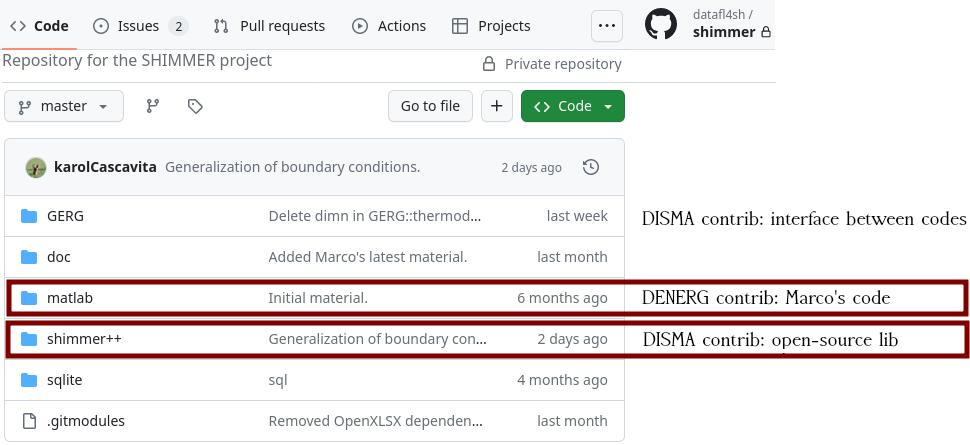
\includegraphics[scale=0.35]{img_other/repo.jpg}
\end{figure}
\item Recommendations:
\begin{itemize}
    \item Do not write in master. Make your branch and make a pull request.
\end{itemize}    
\end{itemize}   
\end{frame}
%----------------------------------------------------------------
\begin{frame}{System boundaries}
\begin{itemize}
    \item Efforts in the in-memory representation and in the numerical methods stages.
\end{itemize}


\begin{figure}[H]
    \centering
    %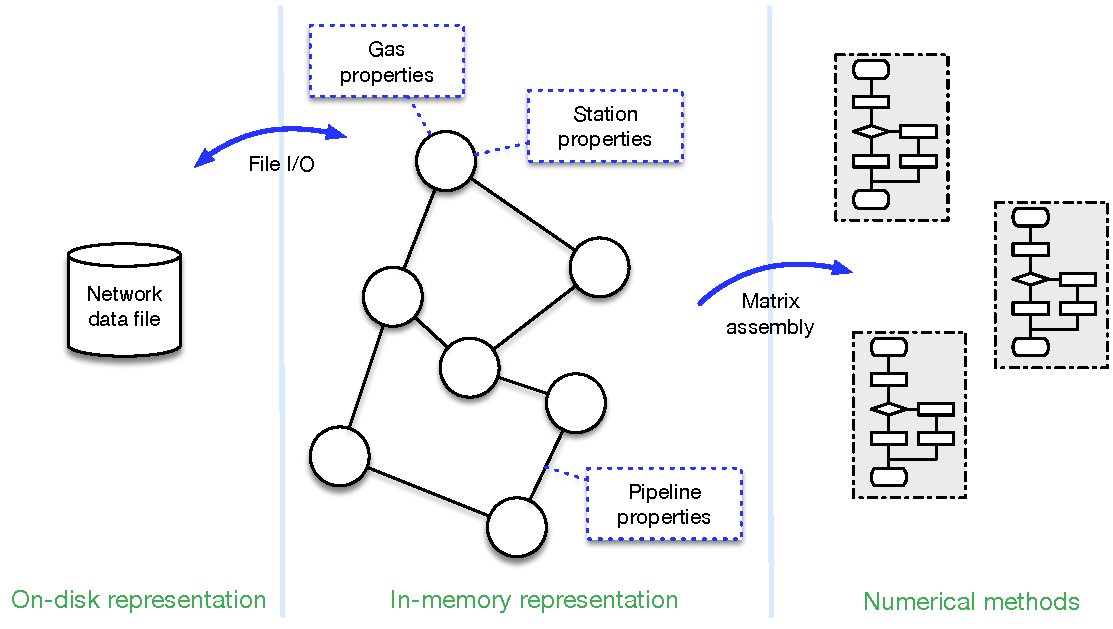
\includegraphics[scale = 0.4]{img_intro/system_arch.pdf}
    \begin{tikzpicture}
    \node[anchor=south west,inner sep=0] (X) at (2, -3) 
    {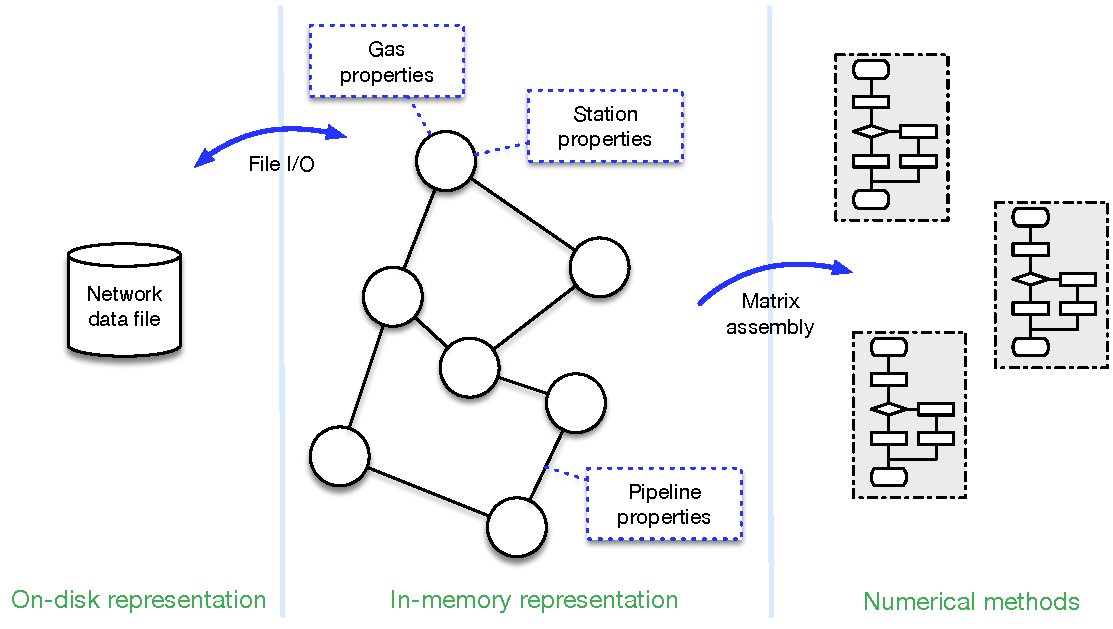
\includegraphics[scale = 0.5]{img_intro/system_arch.pdf}};
    \node [blue, ultra thick] at ($(X.south west)!0.5!(X.north east)$) {};
    % Square for scale 0.4
    %\draw[red] (9.75,-3) -- (9.75,1.25) -- (4.0,1.25) -- (4.0,-3) -- cycle;
    % Square for scale 0.5
    \draw[red] (11.75,-3) -- (11.75,2.25) -- (4.5,2.25) -- (4.5,-3) -- cycle;
    \pgfsetfillcolor{vinotinto}
    \pgfsetfillopacity{0.25}
    \only<2>\fill(8.5,-3) -- (8.5,2.25) -- (4.5,2.25) -- (4.5,-3) -- cycle;   
    \end{tikzpicture}
    \caption{Taken from architecture proposal (Matteo's presentation).}
\end{figure}
   
\end{frame}
